\documentclass[a4paper,french]{article}
\usepackage[latin1]{inputenc}
	\usepackage[T1]{fontenc}
\usepackage{babel} 
\usepackage{etex}
\usepackage{fourier}
\usepackage[table]{xcolor}
\usepackage{tabularx}
\usepackage{cellspace}
	\setlength{\cellspacetoplimit}{4pt}
	\setlength{\cellspacebottomlimit}{4pt}
\usepackage[colorlinks=true,urlcolor=blue]{hyperref}
\usepackage{pas-tableur}
\usepackage{titlesec}
\usepackage{tcolorbox}
	\tcbuselibrary{skins}
	\tcbuselibrary{theorems}
	\tcbuselibrary{breakable}	
\usepackage{listings}
% ----------------------

\usetikzlibrary{arrows}

\setlength{\parindent}{0pt}

\tcbuselibrary{listings}
\usetikzlibrary{decorations.pathmorphing}

% Couleurs utilis�es dans la documentation

\definecolor{codeTitleFont}{cmyk}{0.04,0,0.03,0.16}
\definecolor{codeTitleBackLeft}{cmyk}{0.08,0,0.06,0.76}
\definecolor{codeTitleBackRight}{cmyk}{0.07,0,0.05,0.42}
\definecolor{listingTitleFont}{cmyk}{0,0.31,0.91,0.38}
\definecolor{listingTitleBackLeft}{cmyk}{0,0.05,0.64,0}
\definecolor{listingTitleBackRight}{cmyk}{0,0.03,0.31,0.02}


% Code LaTeX

\tcbset{codeTEX/.style={
	sharp corners=all,
	before skip=1em,
	after skip=1em,
	enhanced,
	frame style={	
			left color=codeTitleBackLeft,
			right color=codeTitleBackRight},
	interior style={
		top color=codeTitleBackLeft!50,
		bottom color=codeTitleBackRight!20},
	boxrule=0.7pt,
	fonttitle={\sffamily\bfseries\color{codeTitleFont}},
	colback=codeTitleFont,
	listing only,
	left=6mm,
	listing options={
		basicstyle=\ttfamily\fontsize{7}{9}\selectfont,
		keywordstyle=\color{blue},
		numbers=left,
		language=TeX,
		breaklines=true,
		morekeywords={definecolor,tcbset,begin, newtcbtheorem,newenvironment,newcommand,bfseries,color, sffamily,tcblower,ttfamily,setlength},
		numberstyle=\tiny\color{red!75!black}},
	breakable
	}
}

% Listing exemples

\tcbset{listing/.style={
	sharp corners=all,
	before skip=1em,
	after skip=1em,
	enhanced,
	frame style={	
			left color=listingTitleBackLeft,
			right color=listingTitleBackRight},
	boxrule=0.7pt,
	fonttitle={\sffamily\bfseries\color{listingTitleFont}},
	colback=listingTitleBackRight,
	breakable,
	listing options={
		basicstyle=\ttfamily\fontsize{7}{9}\selectfont,
		keywordstyle=\color{listingTitleFont},
		numbers=left,
		language=TeX,
		breaklines=true,
		numbersep=5pt,
		morekeywords={ifelse,begin,definecolor,tcbset},
		numberstyle=\tiny\color{red!75!black}},
	},
	interior style={
		draw=listingTitleBackLeft,
		top color=listingTitleBackLeft!50,
		bottom color=listingTitleBackRight!20},
	  segmentation style={
		draw=listingTitleFont,
		solid,
		decorate,
		decoration={random steps,segment length=2mm}
	}
}

% Titre de la documentation

\tcbset{head/.style={
	enhanced,
	hbox,
	tikznode,
	left=8mm,
	right=8mm,
	boxrule=0.4pt,
  colback=white,
  colframe=gray,
  drop lifted shadow=black!50!yellow,
  before=\par\vspace*{5mm},
  after=\par\bigskip,
  interior style={
		draw=white,
		top color=white,
		bottom color=white}
	}
}

% TOC

\tcbset{toc/.style={
	breakable,
	enhanced jigsaw,
	title={\color{red!50!black}Sommaire},
	fonttitle=\bfseries\Large,
  colback=yellow!10!white,
  colframe=red!50!black,
  before=\par\bigskip\noindent,
  interior style={
  	fill overzoom image=goldshade.png,
  	fill image opacity=0.25},
  colbacktitle=yellow!20,
  enlargepage flexible=\baselineskip,
  pad at break*=3mm,
  attach boxed title to top center={
  	yshift=-0.25mm-\tcboxedtitleheight/2,
  	yshifttext=2mm-\tcboxedtitleheight/2},
  boxed title style={
  	enhanced,
  	boxrule=0.5mm,
    frame code={ 
    \path[tcb fill frame] ([xshift=-4mm]frame.west) -- (frame.north west)
    -- (frame.north east) -- ([xshift=4mm]frame.east)
    -- (frame.south east) -- (frame.south west) -- cycle; },
    interior code={ 
    	\path[tcb fill interior] ([xshift=-2mm]interior.west)
    -- (interior.north west) -- (interior.north east)
    -- ([xshift=2mm]interior.east) -- (interior.south east) -- (interior.south west)
    -- cycle;}  },
  drop fuzzy shadow
	}
}

% Historique de l'extension

\tcbset{histo/.style={
	enhanced,
	breakable,
	sidebyside,
	lefthand width=1.5cm
	}
}
\makeatletter

\def\@dottedtocline#1#2#3#4#5{%
  \ifnum #1>\c@tocdepth \else
    \vskip \z@ \@plus.2\p@
    {\leftskip #2\relax \rightskip \@tocrmarg \parfillskip -\rightskip
     \parindent #2\relax\@afterindenttrue
     \interlinepenalty\@M
     \leavevmode
     \@tempdima #3\relax
     \advance\leftskip \@tempdima \null\nobreak\hskip -\leftskip
     {#4}\nobreak
     \leaders\hbox{$\m@th
        \mkern \@dotsep mu\hbox{.}\mkern \@dotsep
        mu$}\hfill
     \nobreak
     \hb@xt@\@pnumwidth{\hfil\helvbx #5}%
     \par}%
  \fi}

\renewcommand*\l@section
{%
\helvbx\color{red!50!black}\bfseries
\def\@linkcolor{red!50!black}\@dottedtocline{1}{1.5em}{1.5em}
}

\renewcommand*\l@subsection
{%
\helvbx\color{green!50!black}
\def\@linkcolor{green!50!black}
\@dottedtocline{1}{2.3em}{2.6em}
}

\renewcommand*\l@subsubsection
{%
\helvbx\color{orange!80!black}
\def\@linkcolor{orange!80!black}
\@dottedtocline{1}{3em}{3.3em}
}

\def\contentsline#1#2#3#4{%
  \ifx\\#4\\%
    \csname l@#1\endcsname{#2}{#3}%
  \else
      \csname l@#1\endcsname{\hyper@linkstart{link}{#4}{#2}\hyper@linkend}{%
        \hyper@linkstart{link}{#4}{#3}\hyper@linkend
      }%
  \fi
}

% --------------------
% TITRES DES SECTIONS 
% --------------------

\titleformat{\section}[block]
{\helvbx\Large\color{red!50!black}}
{\fcolorbox{red!50!black}{red!50!black}{\textcolor{white}{\bfseries\thesection}}}
{1em}
{\helvbx}

\titleformat{\subsection}[block]
{\helvbx\large\color{green!50!black}}
{\thesubsection}
{1em}
{\helvbx}

\titleformat{\subsubsection}[block]
{\helvbx\large\color{orange!50!black}}
{\thesubsubsection}
{1em}
{\helvbx}

\makeatother

\begin{document}

\begin{center}
\begin{tcolorbox}[head]
{\bfseries\LARGE Documentation \texttt{pas-tableur} }\\[3mm]
{\large Version 2.01 -- \today}
\end{tcolorbox}

{\large 
\href{http://www.mathweb.fr/contact.html}{St\'ephane Pasquet}}
\end{center}

\begin{tcolorbox}[toc]
\makeatletter
\@starttoc{toc}
\makeatother
\end{tcolorbox}

\section{Introduction et installation}

L'extension \texttt{pas-tableur.sty} a pour but d'imiter l'apparence des tableurs.

Il ne permet en aucun cas d'effectuer des calculs type tableur.

\medskip

Pour cette version 2 de l'extension, j'ai souhait\'e utiliser une syntaxe dans le fichier sty plus intuitive et plus pratique pour effectuer d'autres op\'erations par rapport \`a la version 1.

\medskip

Cette extension charge automatiquement les extensions suivantes :

\medskip

\begin{quote}
tikz (avec la librairie : calc) \\
xkeyval\\
xstring
\end{quote}

\newpage

On pourra d\'ecompresser \texttt{pas-tableur.zip} 
de sorte \`a avoir :

\begin{itemize}
\item Sous Ubuntu :

\begin{verbatim}
./texlive/texmf-local/tex/latex/pas-tableur/pas-tableur.sty
./texlive/texmf-local/doc/latex/pas-tableur/pas-tableur.tex
./texlive/texmf-local/doc/latex/pas-tableur/pas-tableur.pdf
./texlive/texmf-local/doc/latex/pas-tableur/doc.codes.tex
./texlive/texmf-local/doc/latex/pas-tableur/doc.styles.tex
\end{verbatim}

\item Sous Windows :

\begin{verbatim}
C:\texmf\latex\pas-tableur\pas-tableur.sty
C:\texmf\doc\pas-tableur\pas-tableur.tex
C:\texmf\doc\pas-tableur\pas-tableur.pdf
C:\texmf\doc\pas-tableur\doc.codes.tex
C:\texmf\doc\pas-tableur\doc.styles.tex
\end{verbatim}
\end{itemize}

\medskip

Apr\`es installation, n'oubliez pas de taper la commande \texttt{texhash} dans le terminal pour mettre \`a jour la base de donn\'ees des extensions.

\bigskip 

Sous Mac OS, j'imagine que l'arborescence ressemble \`a ce qui est \'ecrit pr\'ec\'edemment.


\section{\textbackslash tableur et \textbackslash tableur* : construire un tableur}

Pour cr\'eer un tableur, il faudra se mettre dans un environnement \texttt{tikzpicture} et utiliser la commande \textbackslash tableur ou sa version \'etoil\'ee.

\subsection{\textbackslash tableur}

\begin{tcblisting}{codeTEX}
\begin{tikzpicture}
\tableur[<nombre de lignes>]{<colonnes>}
\end{tikzpicture}
\end{tcblisting}

\bigskip

L'argument \og colonnes \fg{} peut se pr\'esenter de deux fa\c cons diff\'erentes :

\bigskip

\begin{tcblisting}{listing,title=Exemple 1}
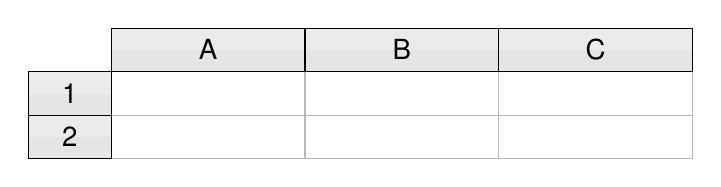
\begin{tikzpicture}
\tableur[2]{A,B,C}
\end{tikzpicture}
\end{tcblisting}

\bigskip

\begin{tcblisting}{listing,title=Exemple 2}
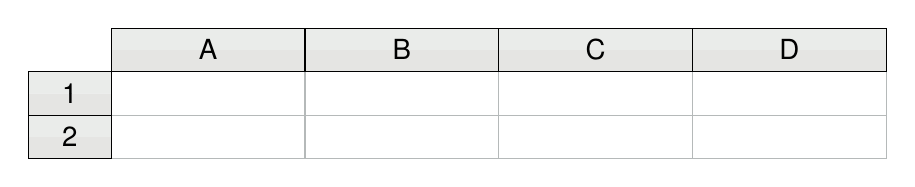
\begin{tikzpicture}
\tableur[2]{A-D}
\end{tikzpicture}
\end{tcblisting}

\bigskip

Pour cette macro, les valeurs par d\'efaut sont :

\medskip

\begin{itemize}
\item la hauteur de chaque ligne : 1.57em ;
\item la largeur de chaque colonne : 7em ;
\item la largeur de la 1\iere{} colonne (contenant le num\'eros des lignes) : 3em ;
\item le nombre de lignes : si l'option entre crochets n'est pas inform\'ee, il y aura 1 ligne.
\end{itemize}

\medskip

Pour changer ces valeurs par d\'efaut, on utilisera les commandes :

\medskip

\begin{tcblisting}{codeTEX}
\tabcolwidth{2cm} % pour que chaque colonne ait une largeur de 2 cm
\tabnumlinewidth{1cm} % pour que la 1\`ere colonne fasse 1 cm de large
\tablineheight{15mm} % pour que chaque ligne ait une hauteur de 15 mm
\end{tcblisting}

\paragraph*{Attention :} il faut imp\'erativement mettre l'unit\'e (cm, mm, em, ex ou pt).

\subsection{\textbackslash tableur*}

La version \'etoil\'ee de \textbackslash\texttt{tableur} permet de construire un tableur dont les colonnes n'ont pas les m\^emes dimensions.


\begin{tcblisting}{listing}
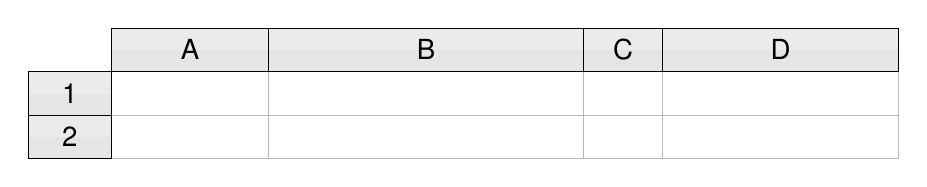
\begin{tikzpicture}
\tableur*[2]{A/2cm,B/4cm,C/1cm,D/3cm}
\end{tikzpicture}
\end{tcblisting}

\newpage

\subsection{Les noms de colonnes}

Les colonnes peuvent porter n'importe quelle lettre majuscule de l'alphabet latin :

ABCDEFGHIJKLMNOPKRSTUVWXYZ.

On ne peut pas nommer les colonnes par \og AA \fg{} par exemple.

\medskip

Quant aux lignes, elles commencent toujours par \og 1 \fg.


\subsection{Les couleurs par d\'efaut}

Deux couleurs sont utilis\'ees pour les cases \og en-t-\^etes \fg{} :

\medskip

\begin{tcblisting}{codeTEX}
\definecolor{grayTopCell}{cmyk}{0.08,0.05,0.06,0}
\definecolor{grayBottomCell}{cmyk}{0.1,0.07,0.08,0}
\end{tcblisting}

\medskip

Pour les changer, vous pouvez les red\'efinir apr\`es avoir appel\'e \texttt{pas-tableur}.

\medskip

Le gris de s\'eparation des cellules est, quant \`a lui, d\'efini par :

\medskip

\begin{tcblisting}{codeTEX}
\definecolor{graySepCell}{cmyk}{0.29,0.21,0.21,0}
\end{tcblisting}

\subsection{La police de caract\`ere des en-t\^ete}

\begin{tcblisting}{codeTEX}
\newcommand{\helvbx}{\usefont{T1}{phv}{m}{n}}
\end{tcblisting}

\medskip

Ainsi, si vous souhaitez ins\'erer le nom d'une cellule dans votre document, vous pouvez utiliser la syntaxe suivante :

\medskip

\begin{tcblisting}{listing}
Dans la cellule {\helvbx A3}, nous 
avons ins\'er\'e la formule...
\end{tcblisting}


\subsection{Nomination des cellules}

Toujours dans un logique de simplifier la r\'edaction des documents, j'ai souhait\'e nommer chaque cellule de fa\c con intuitive.

Ainsi, la cellule {\helvbx A1} est nomm\'ee : cellA-1.

Cette pr\'ecision est utile lorsque l'on souhaite ajouter des fl\`eches vers certaines cellules comme dans l'exemple suivant :

\medskip

\begin{tcblisting}{listing}
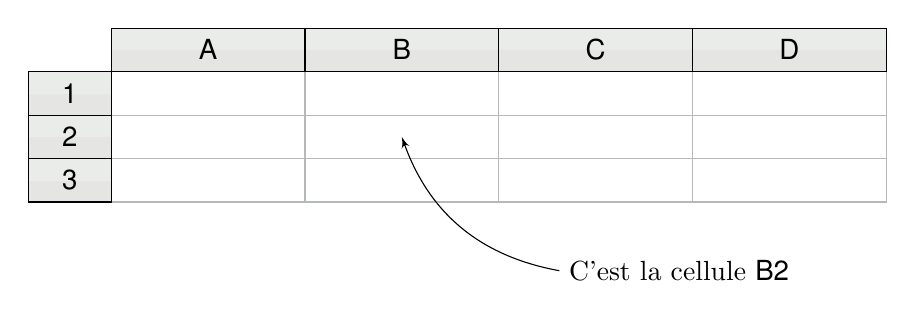
\begin{tikzpicture}
\tableur[3]{A-D}
\draw[<-,>=latex'] (cellB-2.center) to[bend right=30] ($(cellB-2)+(2,-1.7)$) 
node[right] {C'est la cellule {\helvbx B2}};
\end{tikzpicture}
\end{tcblisting}

\section{\textbackslash celtxt et \textbackslash celtxt* : ins\'erer du texte dans une cellule}


\begin{tcblisting}{codeTEX}
% Ins\'erer une formule ou un texte
\celtxt[<options>}{<colonne>}{<ligne>}{<texte>}
% Ins\'erer un texte en mode math\'ematiques ou non
\celtxt*[<options>}{<colonne>}{<ligne>}{<texte>}
\end{tcblisting}

\medskip

Les options sont :

\medskip

\begin{itemize}
\item \texttt{c} : pour centrer le texte ;
\item \texttt{l} : pour positionner le texte \`a gauche (c'est cette valeur qui est d\'esign\'ee par d\'efaut) ;
\item \texttt{r} : pour positionner le texte \`a droite ;

\item \texttt{width=} : pour sp\'ecifier la largeur de la colonne dans le cas o\`u nous avons utilis\'e la commande \texttt{\textbackslash tableur*}. Par d\'efaut,la largeur est 7em (largeur par d\'efaut de chaque colonne) ;

\item \texttt{color=} : couleur du texte. Par d\'efaut, la couleur est noire.
\end{itemize}

\medskip

Le texte peut \^etre format\'e de deux fa\c cons diff\'erentes selon qu'il d\'esigne une formule ou un texte normal, comme le montre l'exemple suivant :

\bigskip

\begin{tcblisting}{listing,title=Exemple 1}
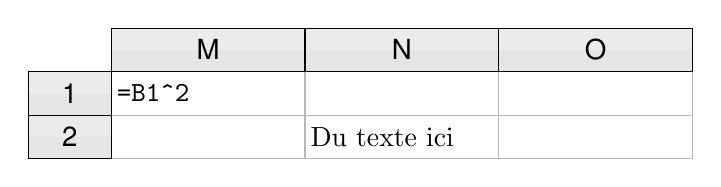
\begin{tikzpicture}
\tableur[2]{M-O}
\celtxt{M}{1}{=B1^2}
\celtxt[r]{N}{2}{Du texte ici}
\end{tikzpicture}
\end{tcblisting}

\medskip

\begin{tcblisting}{listing,title=Exemple 2}
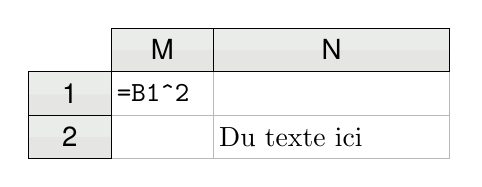
\begin{tikzpicture}
\tableur*[2]{M/13mm,N/3cm}
\celtxt[width=13mm]{M}{1}{=B1^2}
\celtxt[r,width=3cm]{N}{2}
{Du texte ici}
\end{tikzpicture}
\end{tcblisting}

\subsection{Formater le texte}

On peut mettre en italique :

\medskip

\begin{tcblisting}{listing,title=\'Ecrire en italique}
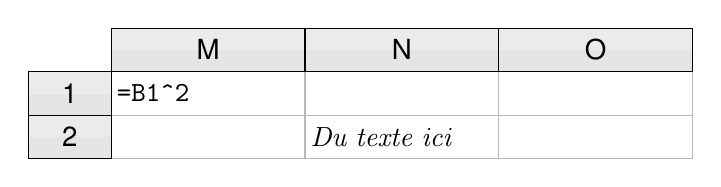
\begin{tikzpicture}
\tableur[2]{M-O}
\celtxt{M}{1}{=B1^2}
\celtxt[r]{N}{2}
{\itshape Du texte ici}
\end{tikzpicture}
\end{tcblisting}

\medskip

ou m\^eme en gras :

\medskip

\begin{tcblisting}{listing,title=\'Ecrire en gras}
\begin{tikzpicture}
\tableur[2]{M-O}
\celtxt{M}{1}{=B1^2}
\celtxt[r]{N}{2}
{\bfseries Du texte ici}
\end{tikzpicture}
\end{tcblisting}

voire m\^eme en petites majuscules :

\medskip

\begin{tcblisting}{listing,title=\'Ecrire en petites majuscules}
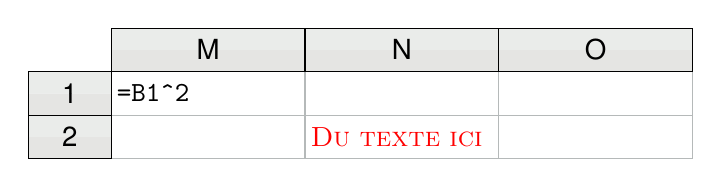
\begin{tikzpicture}
\tableur[2]{M-O}
\celtxt{M}{1}{=B1^2}
\celtxt[r,color=red]{N}{2}
{\scshape Du texte ici}
\end{tikzpicture}
\end{tcblisting}

\subsection{Mode math\'ematique dans une cellule}

G\'en\'eration des premiers termes de la suite d\'efinie par $\left\{\begin{array}{l}
u_0=5\\
u_{n+1}=au_n+0,1
\end{array}
\right.$ o\`u $a$ est une valeur mise dans la cellule \helvbx{
C1}.

\begin{tcblisting}{listing,title=\'Ecrire en mode math\'ematique}
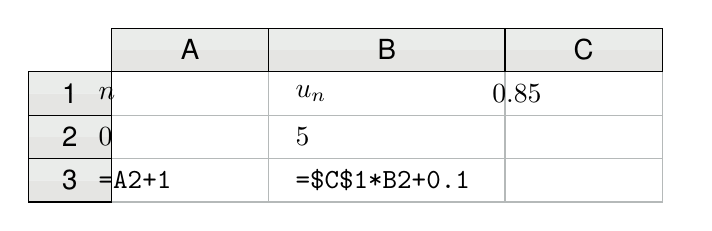
\begin{tikzpicture}
\tableur*[3]{A/2cm,B/3cm,C/2cm}
\celtxt*[c]{A}{1}{$n$}
\celtxt*[c]{B}{1}{$u_n$}
\celtxt[c]{C}{1}{0.85}
\celtxt[c]{A}{2}{0}
\celtxt[c]{B}{2}{5}
\celtxt{A}{3}{=A2+1}
\celtxt{B}{3}{=$C$1*B2+0.1}
\end{tikzpicture}
\end{tcblisting}

\paragraph*{Remarque :} les commandes \texttt{\textbackslash celtxt} et sa version \'etoil\'ee (introduites dans la version 2.01 du 31 janvier 2016) ont \'et\'e r\'e-\'ecrites et imagin\'ees sur la page \url{https://groups.google.com/forum/#!topic/fr.comp.text.tex/7K1r9fUd_Rs}. J'ai donc d\'ecid\'e d'introduire ce nouveau code car il semblerait que certains utilisateurs aient express\'ement envie d'ins\'erer du texte en mode math\'ematique dans certaines cellules.

\section{S\'election de cellules}

\subsection{\textbackslash selecCell : s\'election d'une cellule}

\begin{tcblisting}{codeTEX}
\selecCell{<colonne>}{<ligne>}
\end{tcblisting}

\medskip

Permet de simuler le cas o\`u une cellule est s\'electionn\'ee, comme le montre l'exemple suivant :

\medskip

\begin{tcblisting}{listing}
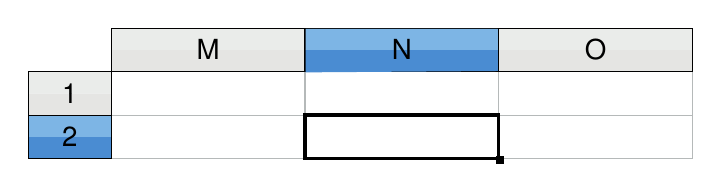
\begin{tikzpicture}
\tableur[2]{M-O}
\selecCell{N}{2}
\end{tikzpicture}
\end{tcblisting}


\subsection{\textbackslash multiSelec : s\'election de plusieurs colonnes}

Voyons un exemple pour comprendre la syntaxe :

\medskip

\begin{tcblisting}{listing}
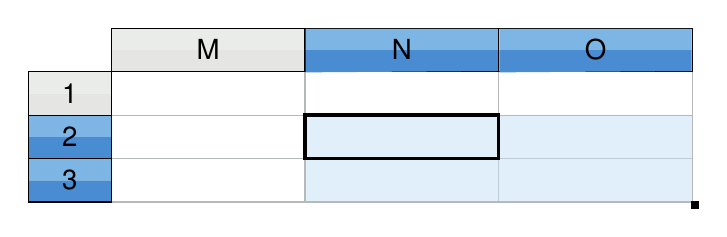
\begin{tikzpicture}
\tableur[3]{M-O}
\multiSelec{N-2}{O-3}
\end{tikzpicture}
\end{tcblisting}

\newpage

\subsection{Les couleurs par d\'efaut}

\begin{tcblisting}{codeTEX}
% Pour les en-tetes
\definecolor{blueSelecCellTop}{cmyk}{0.52,0.17,0,0}
\definecolor{blueSelecCellBottom}{cmyk}{0.75,0.34,0,0}

% Pour les cellules s\'electionn\'ees
\definecolor{blueSelec}{cmyk}{0.23,0.06,0,0}
\end{tcblisting}

\medskip

\`A noter qu'une opacit\'e de 50\,\% est appliqu\'ee pour les cellules s\'electionn\'ees (afin de voir les traits de s\'eparation des cellules).

\section{R\'esum\'e des commandes \`a travers des exemples}

\begin{tabularx}{\linewidth}{|Sl|X|}
\hline
\texttt{\textbackslash tableur[3]\{A-F\}} & Trace un tableur sur 3 lignes, avec les colonnes A, B, C, D, E, F.
\\
\hline
\texttt{\textbackslash tableur[2]\{A,B,C\}} & Trace un tableur sur 2 lignes, avec les colonnes A, B, C.\\
\hline
\texttt{\textbackslash tableur*[3]\{A/2cm,B/5cm\}} & Trace un tableur sur 3 lignes, avec des colonnes A et B de largeur diff\'erente.\\
\hline
\texttt{\textbackslash celtxt[c]\{A\}\{1\}\{=B2*2\}} & Affiche la formule \og =B2*2 \fg{} dans la cellule A1 centr\'ee horizontalement.\\
\hline
\texttt{\textbackslash celtxt[color=red]\{A\}\{1\}\{=B2*2\}} & Affiche en rouge la formule \og =B2*2 \fg{} dans la cellule A1.\\
\hline
\texttt{\textbackslash celtxt[width=5cm]\{A\}\{1\}\{=B2*2\}} & Affiche la formule \og =B2*2 \fg{} dans la cellule A1, de largeur 5 cm.\\
\hline
\texttt{\textbackslash celtxt*[r]\{A\}\{1\}\{\verb+$+u\verb+_+n\verb+$+\}} & Affiche \og $u_n$ \fg{} dans la cellule A1, align\'e \`a droite.\\
\hline
\texttt{\textbackslash selecCell\{A\}\{1\}} & Dessine un cadre autour de la cellule A1.\\
\hline
\texttt{\textbackslash multiSelec\{A-1\}\{C-2\}} & Simule la s\'election des cellules allant de A1 \`a C2.\\
\hline
\texttt{\textbackslash helvbx\{A1\}} & Affiche \helvbx{A1}.\\
\hline
\end{tabularx}

\newpage
\section{Implantation}

\lstset{%
numbers=left,
numberstyle=\tiny,
tabsize=2,
stepnumber=5,
numbersep=5pt,
language=TeX,
breaklines=true,
basicstyle=\small,%
keywordstyle=\color{red!50!black},%
identifierstyle=, %
commentstyle=\color{gray},%
stringstyle=\ttfamily,%
showstringspaces=true,
morekeywords={newcommand,definecolor,RequirePackage, usetikzlibrary,fill,node,draw,tikzstyle,StrChar,StrBetween, foreach,IfSubStr,StrBefore,StrBehind,StrLen,IfBeginWith,makebox, dimexpr,StrGobbleLeft,setlength}}

\lstinputlisting{pas-tableur.sty}

\end{document}